\paragraph{} This chapter aims to identify evidence that the new architectural pattern has improved team productivity and enabled the system to offer functionalities that were not possible with the Fence version. To establish a timeline of events for correlation with the presented data: the Authorship system was deployed in March 2020; following its success, the LHCb Equipment Management System version 2 was released in September 2020; and the Membership Version 2 was released in May 2021.

\section{Cummulative flow chart}
\paragraph{}A Cumulative Flow Diagram (CFD) is a visual tool in Jira Software that tracks the status of project issues over time, providing a dynamic representation of workflow progress. It organizes work items into various statuses (done, blocked, to do, in progress, and in validation), plotted against time on the x-axis and the number of issues on the y-axis, with each area of the chart color-coded to represent different workflow statuses. This diagram is used for identifying workflow bottlenecks by revealing any segments that widen over time, indicating an accumulation of issues. An increase in ``Done" items, such as observed in Figure \ref{fig:cfc_jira} around the release date of the new Authorship and LBEMS systems, on a CFD generally signifies positive developments in project progress and team performance. This trend may indicate enhanced productivity as the team completes tasks more efficiently. It also suggests an effective workflow management strategy, timely meeting of deadlines, and successful issue resolution.

\begin{figure}[H]
    \centering
    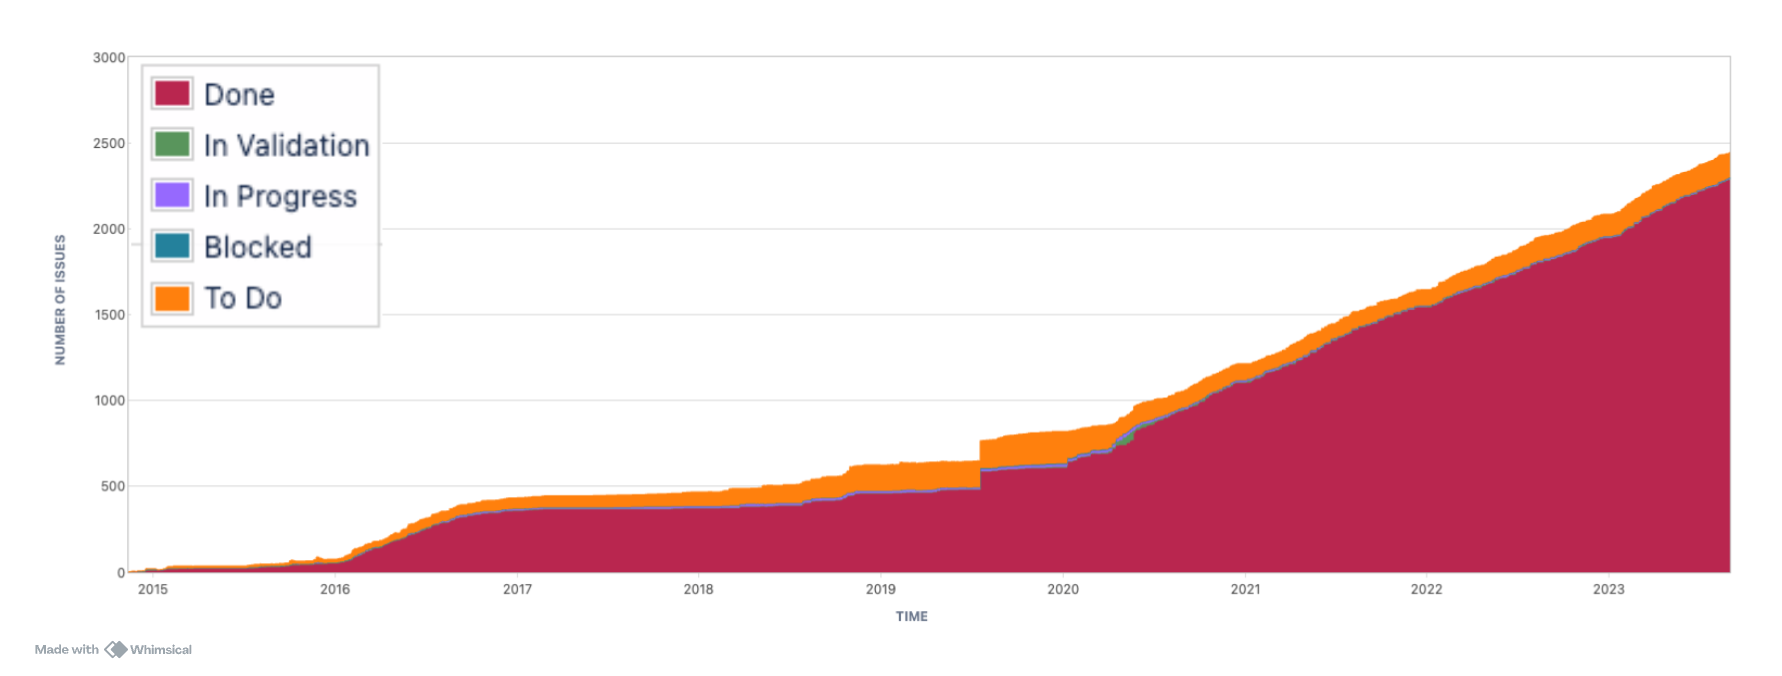
\includegraphics[width=1\linewidth]{figuras/cfd_subtitle.png}
    \caption{CFD graph extracted from Glance's Jira board.}
    \label{fig:cfc_jira}
\end{figure}

\section{Solved versus created report}
\paragraph{} The ``Solved vs.Created" report in Jira is a tool for tracking the rate at which issues are resolved compared to how many are created within a project over a specific period. This report shown in Figure \ref{fig:number_of_issues} plots two lines on a graph: one representing the number of issues created and the other the number of issues solved over time. An upward trend in the ``Solved" line relative to the ``Created" line in this report indicates positive project health and team efficiency. It suggests that the team is effectively addressing and resolving issues faster than new ones are being reported, contributing to the project's forward momentum. Consistently solving more issues than are created can lead to increased stakeholder confidence, as it demonstrates the team's capacity to handle challenges and maintain control over the project's scope. In Figure \ref{fig:number_of_issues} it is possible to notice an inflection point around the Authorship and LBEMS release dates, indicating performance gains by using the new architecture.

\begin{figure}[H]
    \centering
    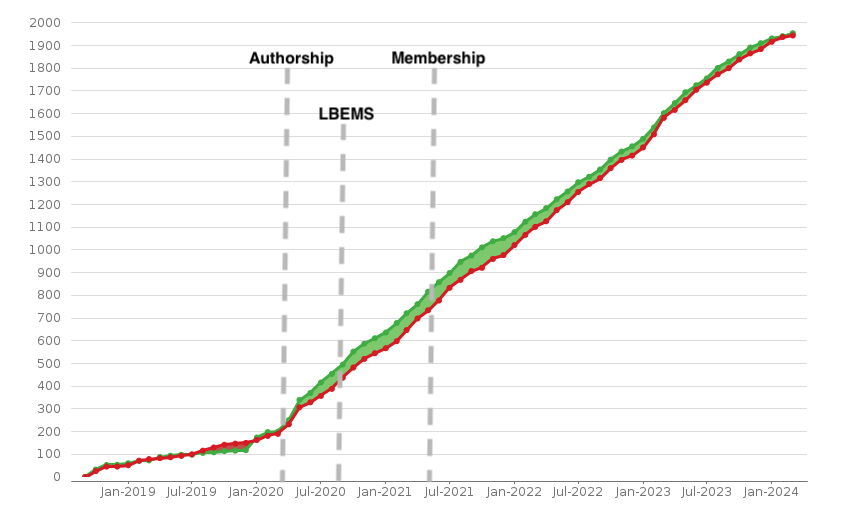
\includegraphics[width=0.7\linewidth]{figuras/number_of_issues_2.png}
    \caption{Solved vs. Created issues in the LHCb Glanace systems.}
    \label{fig:number_of_issues}
\end{figure}

\paragraph{} A pie chart displaying the distribution of issue types within a Jira Software project provides a visual breakdown of where the team's efforts are being allocated, categorizing issues into types such as stories, bugs, tasks, etc. An increase in the percentage of story issues and a decrease in the percentage of bug issues, as depicted in Figure \ref{fig:pie_jira}, can offer observations into the project's current phase and overall health. The shift towards a higher proportion of story issues as observed in Figure \ref{fig:pie_jira} might suggest that the project is in a phase of active development or feature expansion, with the team focusing more on adding new functionalities or enhancements. On the other hand, a decrease in the percentage of bug issues could signal improvements in the quality of the codebase or the effectiveness of the project's quality assurance processes.

\begin{figure} [H]
    \centering
    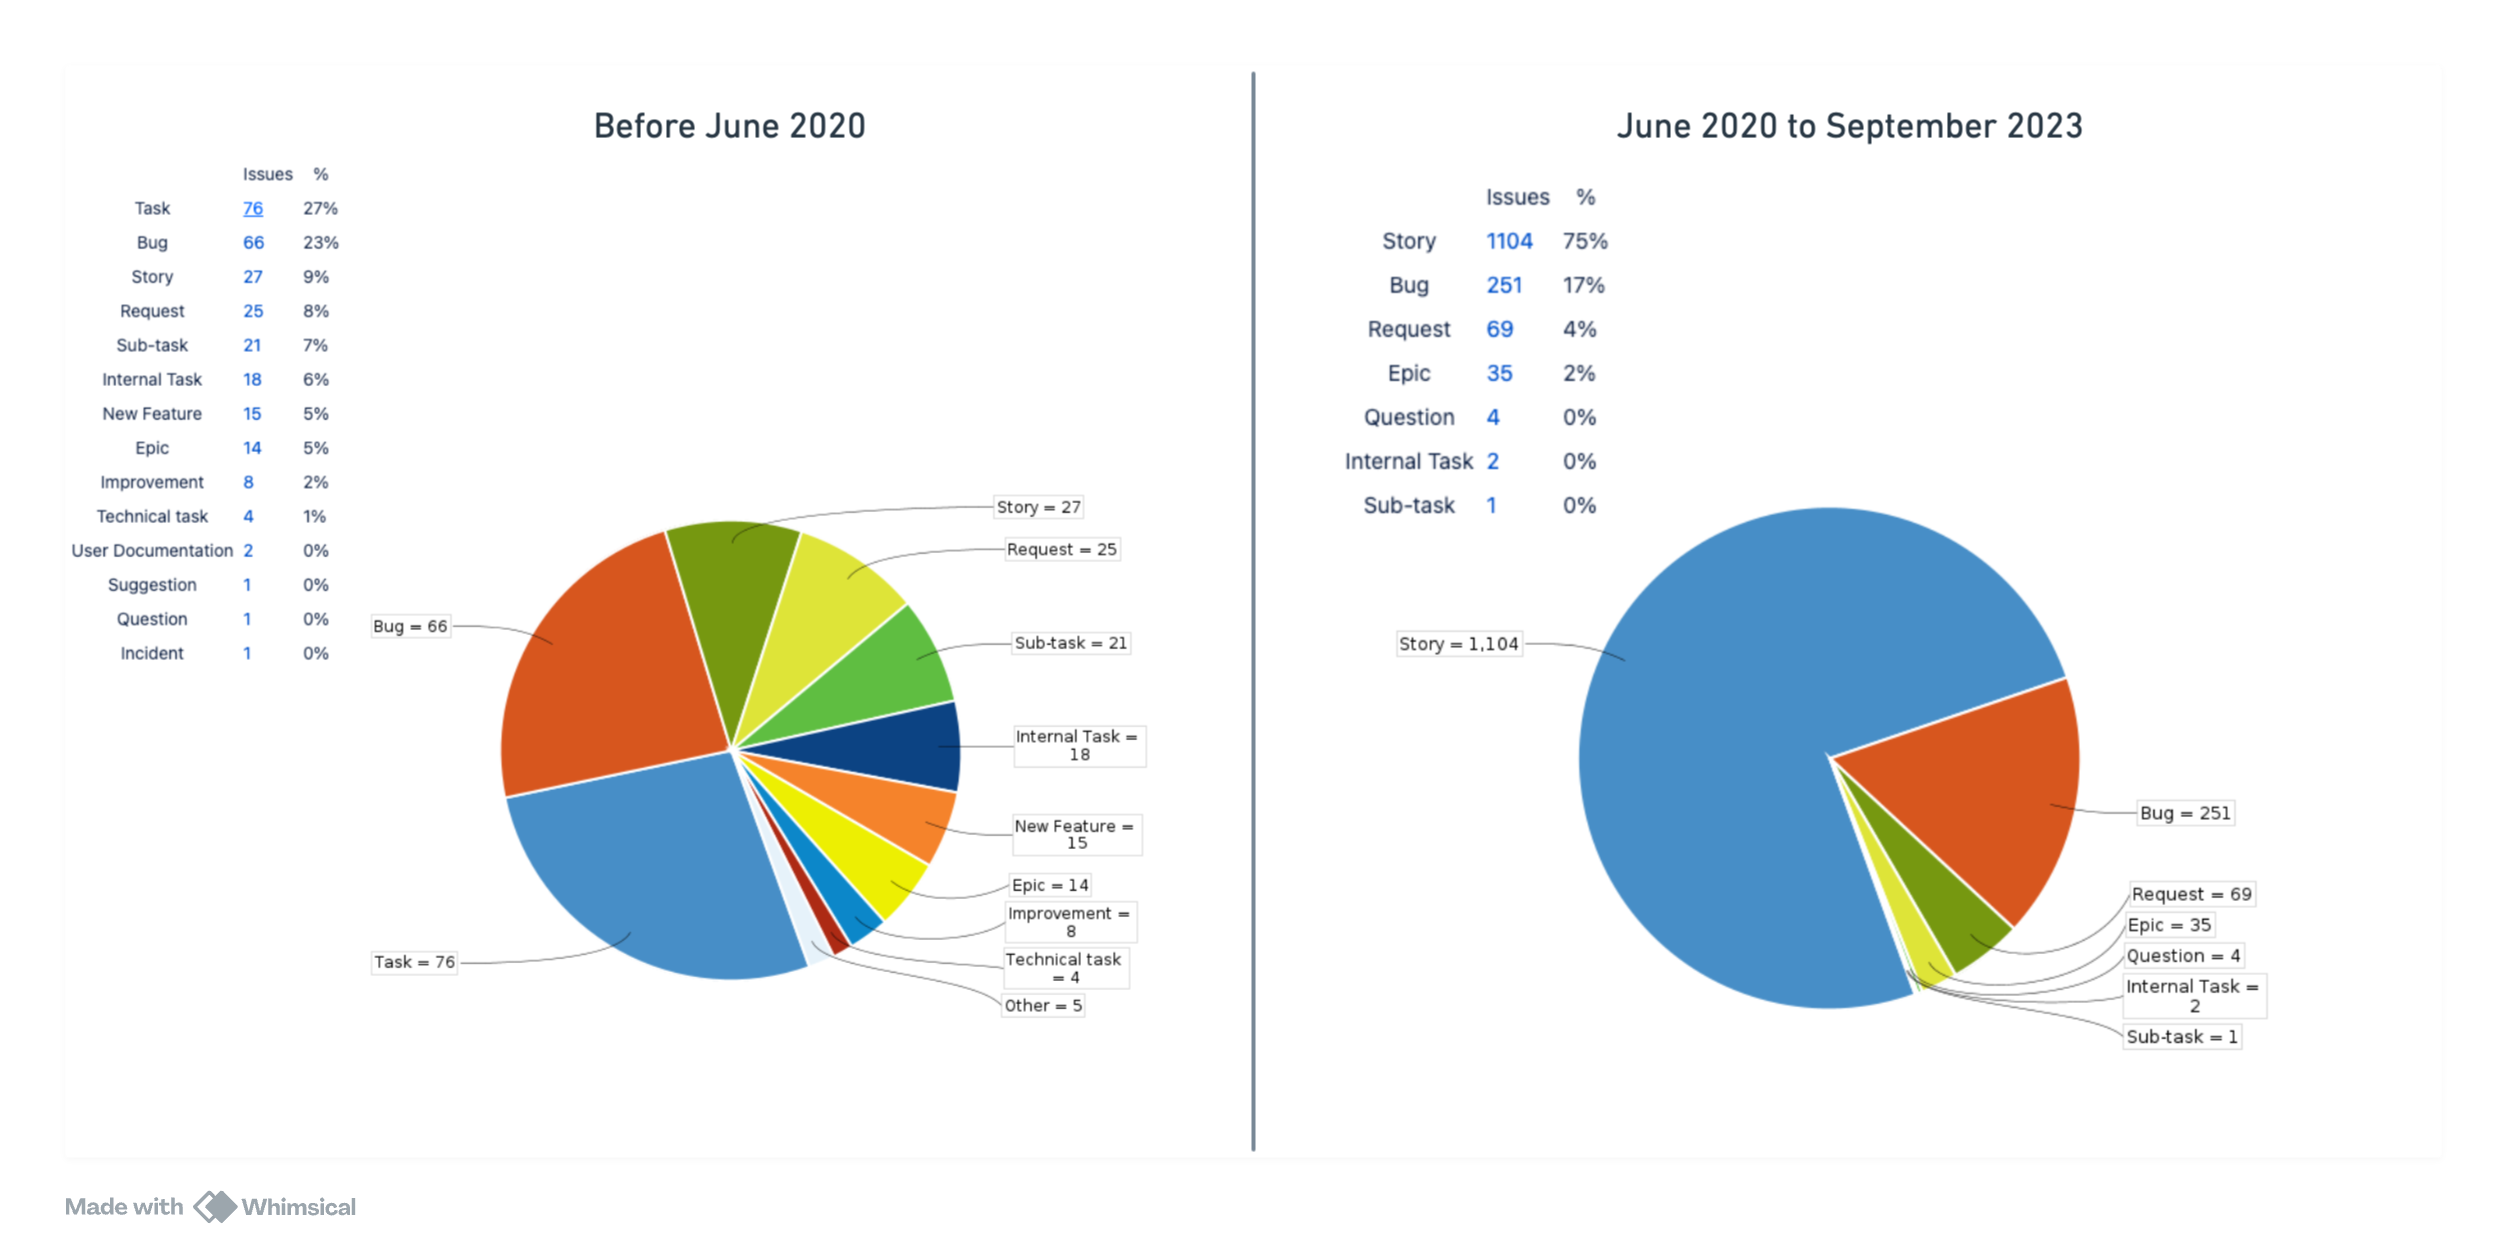
\includegraphics[width=1\linewidth]{figuras/pie_jira_2.png}
    \caption{Issues according to their type.}
    \label{fig:pie_jira}
\end{figure}






\section{Test coverage}
\paragraph{} In the version of the Membership system powered by Fence, automated testing was absent. With the introduction of a decoupled architecture in the subsequent iteration, automated integration testing was established to verify the stability of API endpoints against code alterations. Integration of these tests with Gitlab CI ensures that merge requests are only approved subsequent to the successful completion of all tests. This strategy, prioritizing integration tests, was influenced by the observation that modifications to the database and persistence layers were predominantly responsible for breaking changes. The distribution of test cases across different classes is illustrated in Table \ref{table:test_classes_and_numbers}.



\begin{longtable}{|p{0.5\textwidth}|p{0.4\textwidth}|}
\caption{Test Classes and Number of Tests}\label{table:test_classes_and_numbers}\\
\hline
\textbf{Test Class} & \textbf{Number of Tests} \\ \hline
\endfirsthead

\multicolumn{2}{c}%
{{\bfseries \tablename\ \thetable{} -- continued from previous page}} \\
\hline
\textbf{Test Class} & \textbf{Number of Tests} \\
\hline
\endhead

\hline
\endlastfoot

AppointmentTest.php & 12 \\
AuthorsListTest.php & 7 \\
CountryTest.php & 6 \\
EmploymentTest.php & 15 \\
GrantTest.php & 8 \\
InstituteTest.php & 11 \\
MemberTest.php & 14 \\
NewcomerTest.php & 10 \\
ParticipationTest.php & 4 \\
ReportTest.php & 3 \\
WorkflowTest.php & 27 \\
\end{longtable}



\section{Adoption by external systems}
\paragraph{} Two other web applications at CERN rely on Member information: the Speakers Bureau system, which assigns members to available talks and workshops, and the LHCb Shift system, which allocates members to shifts in the LHCb detector control room to assist in the 24/7 monitoring of the detector's operation. Prior to Membership Version 2, extracting data automatically from the Membership system was feasible only via direct database access, potentially violating OC11 regulations. Consequently, these systems would often maintain their internal lists of Members and Institutes, resorting to manual synchronization with the Membership database—the authoritative source for this data.

\paragraph{} The launch of Membership Version 2, which now offers a REST API, has significantly streamlined the process for related systems at CERN. These systems no longer require maintaining internal databases; instead, they directly access Member and Institute information via specific API endpoints. They can internalize this data through if needed and employ a polling mechanism to periodically refresh the information. To encourage and simplify integration, the Glance team developed a basic Python SDK (software development kit), recognizing that both applications are Python-based. This SDK abstracts the authentication and API call process, allowing for straightforward data retrieval through the \verb|search_member| method with the necessary search parameters. Listing \ref{lst:mb_sdk} showcases the \verb|search_member| function being used to find a specific member based on their CERN identifier. Listing \ref{lst:mb_sdk_implement} displays the \verb|search_member| method implementation, utilizing the \verb|get_api_access_token| function, also provided by the SDK, to retrieve the bearer token required for communicating with the Membership API.

\begin{lstlisting}[language=python, caption=Membership Python SDK usage., label=lst:mb_sdk]
from search_members import search_members

print(search_members(
    offset = 0,
    limit = 10,
    queryString = '"personId" =  "840720"'
    )
)

\end{lstlisting}

\begin{lstlisting}[language=python, caption=Membership SDK implementation., label=lst:mb_sdk_implement]
def search_members(offset, limit, queryString):
    load_dotenv()
    target_client_id = os.getenv('TARGET_CLIENT_ID')
    client_id = os.getenv('CLIENT_ID')
    client_secret = os.getenv('CLIENT_SECRET')
    api_base_url = os.getenv('API_BASE_URL')

    try:
        api_token = get_api_access_token(client_id, client_secret, target_client_id)
    except Exception as e:
        raise(Exception('Token exchange failed. Please check the user and the application credentials'))

    queryString = urllib.parse.quote_plus(queryString)
    url=f'{api_base_url}/members/search?offset={offset}&limit={limit}&queryString={queryString}'
    headers = {'Authorization': f'Bearer {api_token}'}
    #In case you need to use a proxy, uncomment both the following line and also the one on the request. You also need to set your proxy address and port
    #proxies = {"https": "http://127.0.0.1:54321"}

    try:
        response = requests.get(
            url,
            headers=headers,
            verify=False,
            #proxies=proxies
        )
    except Exception as e:
        print(e)
        raise(Exception('API call failed. Please check the API endpoint'))
    return response.json()
\end{lstlisting}




%\section{User experience survey}
%\subsubsection{Features}
%Whether or not the new version includes more useful features when compared to the old version

%\subsubsection{Look and Feel / Performance}
%How do you prefer the current look and feel when compared to the old one?

%\subsubsection{Stability}
%How often do you encounter unexpected behaviors when compared to the previous version? 

\section{Acknowledgements}

\paragraph{} A noteworthy and subjective outcome was the marked improvement in user satisfaction with the newly implemented systems. By employing Domain-Driven Design, developers were able to create features more closely aligned with real-life processes rather than generic, contextless CRUD operations. This enhancement in functionality received recognition in significant collaboration meetings, as illustrated in Figure \ref{fig:reconhecimentos}, underscoring the Glance team's growing significance at CERN and affirming the efficacy of the new architecture.

\begin{figure}[H]
    \centering
    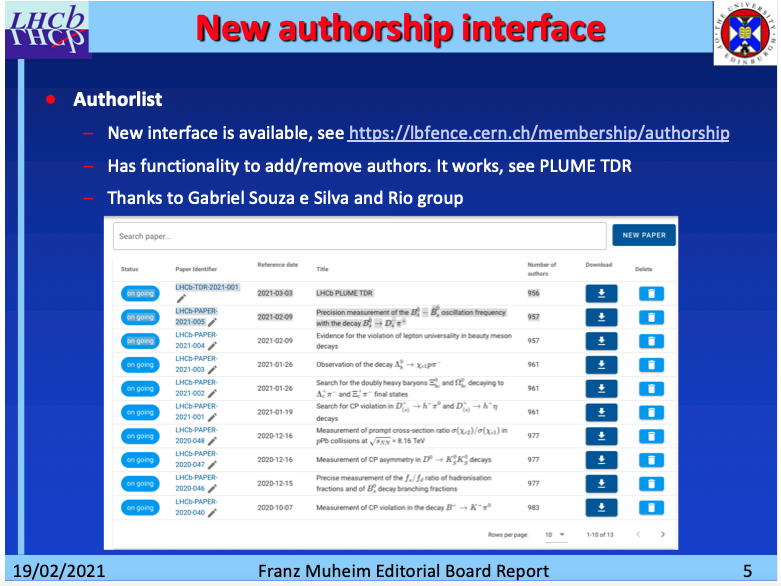
\includegraphics[width=1\linewidth]{figuras/reconhecimentos.png}
    \caption{Acknowledgement.}
    \label{fig:reconhecimentos}
\end{figure}



